\subsection{Modes in Waveguides}\label{sec:modes_tem_cell}
\subsubsection{Rectangular Waveguides as non-TEM structures}




\begin{figure}[htbp]
	\centering
	\begin{subfigure}[b]{0.45\textwidth}
			\centering
		\includegraphics[width=1\linewidth]{content/img/rect_waveguide_tm}
		\caption{TM\textsubscript{11} mode}
		\label{fig:rectwaveguidetm}
	\end{subfigure}
	\hfill
	\begin{subfigure}[b]{0.45\textwidth}
	\centering
\includegraphics[width=1\linewidth]{content/img/rect_waveguide_te}
\caption{TE\textsubscript{10} mode}
\label{fig:rectwaveguidete}
	\end{subfigure}
	
	\caption{Dominant modes in a rectangular waveguide.}
	\label{fig:rect_waveguide_modes}
\end{figure}


A hollow rectangular waveguide with perfectly conducting walls cannot support TEM modes. This can be shown directly from Maxwell's equation, as done in \cite[pp. 425-427]{Griffiths_2024}. The first two dominant modes are demonstrated in \autoref{fig:rect_waveguide_modes}. The electric field intensity $\mathbf{E}$ and magnetic field intensity $\mathbf{H}$ are defined as 

\begin{subequations}
	\begin{align}
		\mathbf{E}&=(E_{0,x}\cdot\mathbf{\hat{a}}_x+E_{0,y}\cdot\mathbf{\hat{a}}_y+E_{0,z}\cdot\mathbf{\hat{a}}_z)\mathrm{e}^{-jkz},\label{eqn:rect_e}\\
		\mathbf{H}&=(H_{0,x}\cdot\mathbf{\hat{a}}_x+H_{0,y}\cdot\mathbf{\hat{a}}_y+H_{0,z}\cdot\mathbf{\hat{a}}_z)\mathrm{e}^{-jkz}.\label{eqn:rect_h}
	\end{align}
\end{subequations}

Using Faraday's and Ampère-Maxwell law transforms \crefrange{eqn:rect_e}{eqn:rect_h} to

\begin{subequations}
\begin{align}
	\nabla \times \mathbf{E} &=\begin{pmatrix}\frac{\mathrm{d}}{\mathrm{d}y}E_z-\mathrm{i}kE_y \\\mathrm{i}kE_x-\frac{\mathrm{d}}{\mathrm{d}x}E_z \\\frac{\mathrm{d}}{\mathrm{d}x}E_y-\frac{\mathrm{d}}{\mathrm{d}y}E_x\end{pmatrix}=\begin{pmatrix} -\mathrm{i}\omega B_x\\-\mathrm{i}\omega B_y\\ -\mathrm{i}\omega B_z \end{pmatrix}\label{eqn:faraday},\\
	\nabla \times \mathbf{B} &=\begin{pmatrix}\frac{\mathrm{d}}{\mathrm{d}y}B_z-\mathrm{i}kB_y \\\mathrm{i}kB_x-\frac{\mathrm{d}}{\mathrm{d}x}B_z \\\frac{\mathrm{d}}{\mathrm{d}x}B_y-\frac{\mathrm{d}}{\mathrm{d}y}B_x\end{pmatrix}=\begin{pmatrix} \frac{\mathrm{i}\omega}{\mu\epsilon} E_x\\\frac{\mathrm{i}\omega}{\mu\epsilon} E_y\\ \frac{\mathrm{i}\omega}{\mu\epsilon} E_z \end{pmatrix}.\label{eqn:ampere_maxwell}
\end{align}
\end{subequations}

For a TEM mode, the longitudinal field components vanish $E_\mathrm{z}=H_\mathrm{z}=0$. Under this assumption, \crefrange{eqn:faraday}{eqn:ampere_maxwell} together with the Gauss' law and Faraday's law reduce to the following conditions for $\mathbf{E}$ components:

\begin{align}
	\frac{\mathrm{d}}{\mathrm{d}x}E_x+\frac{\mathrm{d}}{\mathrm{d}y}E_y&=0\quad\text{Derived out of Gauss' law}\label{eqn:rect_waveguide_gauss},\\
	\frac{\mathrm{d}}{\mathrm{d}y}E_x-\frac{\mathrm{d}}{\mathrm{d}x}E_y&=0\quad\text{Derived out of Faraday's law}\label{eqn:rect_waveguide_faraday}.
\end{align}

The derived \crefrange{eqn:rect_waveguide_gauss}{eqn:rect_waveguide_faraday} cannot fulfill any boundary conditions imposed by the rectangular waveguide. Therefore, a TEM mode cannot propagate.

\subsubsection{TEM mode in the TEM cell}

Opposed to the rectangular waveguide, a TEM cell conducts TEM waves. Further, the TEM mode is necessarily excited by the geometry of the TEM cell, hence this mode is called essential. The higher order TE and TM modes, which are only excited due to non-uniformity of the TEM cell, are called non-essential modes \cite{990711}.

%Additionally, it shields the waves from radiating to the sides, which is advantageous over a stripline \cite{809846,990711}. 

The TEM mode in the TEM cell is derived by a procedure presented in \cites{Tippet_Chang_Crawford_1976,Wilson_1981}. It consists of finding the Green's function of both the TE and TM modes transverse field components $H_z, E_z$ in a rectangular waveguide. The Green's function fulfills the wave equations and boundary conditions of the waveguide, constructed as discussed in \cref{sec:scal_green}, with 

\begin{subequations}
	
	\begin{equation}
		(\nabla^2 + k_{0,t}^2) G (\mathbf{x}_t, \mathbf{x}_t') = -\delta(\mathbf{x}_t - \mathbf{x}_t'),
	\end{equation}
	
	\begin{equation}
		\frac{\partial G(\mathbf{x}_t, \mathbf{x}_t')}{\partial\mathbf{n}}=0.
		\label{eqn:bc_tem} 
	\end{equation}

\end{subequations}

The wave number is separated in a transversal and a longitudinal component $k_0^2=k_{0,t}^2+k_{0,z}^2$. \autoref{eqn:bc_tem} express the boundary condition on the perfectly conducting walls and septum of the TEM cell\todo{sketch}, as well as for the gaps. The source points are denoted with $\mathbf{x'}_t=(\mathbf{\hat{a}}_xx'+\mathbf{\hat{a}}_yy')$ and the observation points with $\mathbf{x}_t=(\mathbf{\hat{a}}_xx+\mathbf{\hat{a}}_yy)$. They are transformed, such that they have a dependence on the wave number $k$ instead of a $z$-dependence. This significantly facilitates the derivation of the Green's function, since only a two-dimensional surface has to be considered. 

The source exciting the waveguide is assumed to be an infinitesimal electric dipole moment centrally located and oriented along the $y$-axis. 
Solving for $H_z$ and applying Green's second identity yields

\begin{align}
	\int_l \left( G(\mathbf{x}_t, \mathbf{x}_t') \frac{\partial H_z(\mathbf{x}_t)}{\partial\mathbf{n}} - H_z(\mathbf{x}_t){\frac{\partial G(\mathbf{x}_t, \mathbf{x}_t')}{\partial\mathbf{n}}}\right)\,&d\mathbf{l'} =\\ = H_z(\mathbf{x}_t)-\int_S J_y(\mathbf{x'}_t)\frac{\partial G(\mathbf{x}_t, \mathbf{x}_t')}{\partial\mathbf{x'}_t}\,&d\mathbf{S}',
	\label{eqn:second_green}
\end{align}

where $S$ is the surface of the waveguide cross section, and $l$ is its boundary. Applying the boundary condition on the perfectly conducting septum and walls, leaves the boundary integrals along the gaps. Further, inserting the electric dipole in \autoref{eqn:second_green} and forcing $H_z$ to be continuous across the gaps leads to 

 \begin{equation}
 		\int_\mathrm{gaps} G(\mathbf{x}_t, \mathbf{x}_t') \frac{\partial H_z(x',0)}{\partial y'}\,dx' = -\mathbf{m}_e \frac{\partial G(\mathbf{x}_t, \mathbf{x}_t')}{\partial\mathbf{x'}_t}.
 \end{equation}

Solving for the Green's function $G$ yields a solution for the magnetic longitudinal field intensity $H_z$ of the TE mode. The same process can be applied to solve for the electric longitudinal field intensity $E_z$ of the TM mode. The total field distribution is a superposition of the TE and TM mode fields, which finally demonstrates the excitation of the TEM mode. The transversal fields $E_t$, $H_t$ relate to $H_z$ with 

\begin{subequations}
	\begin{equation}
		E_t(\mathbf{x}_t) = \frac{j\omega\mu_0}{k_{0,t}^2}\, \frac{\partial H_z(\mathbf{x}_t)}{\partial \mathbf{t}} \times \mathbf{\hat{a}}_z,
	\end{equation}
	\begin{equation}
		H_t(\mathbf{x}_t) = \frac{j k_{0,z}}{k_{0,t}^2} \frac{\partial H_z(\mathbf{x}_t)}{\partial \mathbf{t}},
	\end{equation}
\end{subequations}

and to $E_z$ with

\begin{subequations}
	\begin{equation}
		E_t(\mathbf{x}_t) = \frac{j k_{0,z}}{k_{0,t}^2}\frac{\partial{E}_z(\mathbf{x}_t)}{\partial \mathbf{t}},
	\end{equation}
	\begin{equation}	
		H_t(\mathbf{x}_t) = \frac{-j\omega\epsilon_0}{k_{0,t}^2}  \frac{\partial E_z(\mathbf{x}_t)}{\partial \mathbf{t}} \times \mathbf{\hat{a}}_z,
	\end{equation}
\end{subequations}

where $\mathbf{t}$ denotes the transversal unit vector.

%
%A TEM cell solves this problem, by having a gap between the septum and the side walls. Essentially, it can be considered as two rectangular waveguides with apertures on the sides. Those apertures allow perturbations of the electromagnetic fields between them. The boundary conditions of the Laplace equation now changed due to the gaps. The Green's function may be calculated of the new construction, now considering the boundary conditions at the gaps, which must be the same for both waveguides (to prevent discontinuities). In the papers of Tippet, Chang and Wilson, this new Green's function lead to the excitation of TEM modes in both waveguides \cite{Tippet_Chang_Crawford_1976,Wilson_1981}.
%
%Constraints in their involve the gap is assumed to be small, electrically ($\xi g \ll 1$) and compared to the septum width ($g/a \ll 1$) \cite{4091747}. The variable $\xi=\sqrt{k_0^2 - \beta ^2}$ is the transverse (in y-direction) propagation constant, and consists of the free-space wave number $k_0$ and longitudinal (in z-direction) propagation constant $\beta$. The variables $g$ and $a$ are geometry variables of the TEM cell annotated in \autoref{fig:verticalantennatemcell}.


\subsubsection{Higher-order modes}

The TEM cell under investigation has a width of $a=40\,\mathrm{mm}$ and a height of $b=24\,\mathrm{mm}$. A cross section of the TEM cell with the important dimensions is shown in \autoref{fig:tem_cell_crosssection}. For a thin septum ($t/b \ll 0.1$), the cut-off frequency $f_\mathrm{c}$ of modes with n-even subscripts, i.e. TE\textsubscript{m,2n} and TM\textsubscript{m,2n} modes, is approximated as 

\begin{equation}
	f_c = \frac{c}{2} \sqrt{\left(\frac{m}{a}\right)^2 + \left(\frac{n}{b}\right)^2}.
	\label{eqn:cutoff_frequency_rect_waveguide}
\end{equation}

\begin{itemize}
	\item \( f_c \): cutoff frequency of the mode \(\text{T}_{mn}\)
	\item \( c \): speed of light in the medium (approximately \(3 \times 10^8 \, \text{m/s}\) in air)
	\item \( a \): wider dimension (broad wall) of the rectangular waveguide (meters)
	\item \( b \): narrower dimension (narrow wall) of the rectangular waveguide (meters)
	\item \( m \): mode index in the \(a\)-direction (integer, \(m \geq 0\))
	\item \( n \): mode index in the \(b\)-direction (integer, \(n \geq 0\))
\end{itemize}

\autoref{eqn:cutoff_frequency_rect_waveguide} is also valid for $f_\mathrm{c}$ of higher-order modes in rectangular waveguides \cite{Weil_Gruner_1984}.

\begin{figure}[h]
	\centering
	\includegraphics[width=0.5\linewidth]{content/img/tem_cell_crosssection.png}
	\caption{Geometrical arrangement of the TEM cell in the xy-plane.}
	\label{fig:tem_cell_crosssection}
\end{figure}

The cutoff frequency of the TE\textsubscript{10} mode equals $f_\mathrm{c,10}=3.75\,\mathrm{GHz}$, according to \autoref{eqn:cutoff_frequency_rect_waveguide}. A numerical approach yields the forward transmission coefficients between the output ports of the TEM cell S\textsubscript{12} shown in \autoref{fig:te01_te10_tem_propagation}. There, the cut-off frequency $f_\mathrm{c}$ is defined as the smallest frequency point of undisturbed mode propagation (S\textsubscript{12}$=0\,\mathrm{dB}$). 

\todo[inline]{Note for potential further work in this chapter: A paper by Wilson and Ma present analytical approximations to determine the cut-off frequencies \cite{Wilson_Ma_1986}.  There is a long list for the several first few corner frequencies of the first modes. Additionally, a paper by Koch, Groh and Garbe determines the resonance frequencies of the first TE modes analytically \cite{10791592}. }

A TEM cell contains a tapered section at the output ports. TEM modes pass this section with a minimal amount of reflections. However, higher order TE and TM modes reflect from those sections, and because the TEM cell is a high-Q cavity, resonances occur at $\frac{\lambda}{4}$ and $\frac{\lambda}{2}$ \cite{990711}.\todo[inline]{Simulations with a tapered section have been done in \cite{990711}}

\begin{figure}[h]
	\centering
	\includegraphics[width=0.5\linewidth]{content/img/tem_cell_modes.png}
	\caption{Propagation of TEM, TE\textsubscript{01} and TE\textsubscript{10} modes in the TEM cell. 
		The black trace shows the S\textsubscript{12}-parameter over the frequency of TEM mode. The blue trace demonstrates S\textsubscript{12}-parameter of the TE\textsubscript{10} mode. At a frequency of 3.75\,GHz, this mode propagates without attenuation (S\textsubscript{12}$=0$), defining the cut-off frequency $f_\mathrm{c,10}$. The simulated result comes very close to the analytically determined one. The red trace shows a cutoff frequency of $f_\mathrm{c,10}=3.12\,\mathrm{GHz}$ for the TE\textsubscript{01} mode. \autoref{eqn:cutoff_frequency_rect_waveguide} would predict a cutoff frequency of 6.25\,GHz, however, the septum influences n-odd modes like this one. Their cutoff frequencies are shifted to a lower value \cite{Weil_Gruner_1984}.}
	\label{fig:te01_te10_tem_propagation}
\end{figure}

\todo[inline]{plot title: $|S_{12}|$}

Due to imperfections, change in materials or finite conductivity of the conducting plates, wave propagating in the TEM mode may excite higher order TE and TM modes \cite{10791592}. A change in material, for example, demands the electric and magnetic field to have a component in the direction of propagation at the discontinuity, consequently exciting TM modes. 

The TE\textsubscript{10} and TE\textsubscript{01} modes are non-essential modes with the lowest cut-off frequencies. Their transversal electric fields are depicted in \autoref{fig:transversal_e_fields_tem_cell}. 

\begin{figure}[h]
	\centering
	\begin{subfigure}[b]{0.3\linewidth}
		\centering
		\includegraphics[width=\linewidth]{content/img/tem_cell_mode.png}
		\caption{TEM Mode}
		\label{fig:tem_mode}
	\end{subfigure}
	\begin{subfigure}[b]{0.3\linewidth}
		\centering
		\includegraphics[width=\linewidth]{content/img/te01_mode.png}
		\caption{TE\textsubscript{01}}
		\label{fig:te01_mode}
	\end{subfigure}
	\begin{subfigure}[b]{0.3\linewidth}
		\centering
		\includegraphics[width=\linewidth]{content/img/te10_mode.png}
		\caption{TE\textsubscript{10}}
		\label{fig:te10_mode}
	\end{subfigure}
	\caption{Transversal electric fields in cross section of TEM cell}
	\label{fig:transversal_e_fields_tem_cell}
\end{figure}

\autoref{tab:modes_tem_cell} shows some cut-off frequencies of these modes for different TEM cell dimensions. A characteristic impedance of $50\,\Omega$ at the output ports is only kept in the case $a=40\,\mathrm{mm}$ and $b=24\,\mathrm{mm}$.  

\begin{table}[h]
	\centering

	\begin{tabular}{|c|c||c|c|}
		\hline
		$a$ (mm)& $b$ (mm)&TE\textsubscript{01} $f_\mathrm{c}$ (GHz) &TE\textsubscript{10} $f_\mathrm{c}$ (GHz)\\
		\hline\hline
		80 & 24 & 1.89 & 2.05 \\
		\hline\hline
		40 & 24 & 3.17 & 3.76 \\
		\hline\hline
		40 & 48 & 2.10 & 3.76 \\
		\hline
	\end{tabular}
	\caption{Cut-off frequencies of higher order modes at different TEM cell dimensions. The TE\textsubscript{10}-mode is independent of the height $b$ of the TEM cell, as would be the case in a rectangular waveguide. Both the TE\textsubscript{10}-mode and the TE\textsubscript{01}-mode are dependent on the width $a$. }
	
	\label{tab:modes_tem_cell}
\end{table}

\FloatBarrier
\subsubsection{Field distributions}\label{sec:field_dist}
\FloatBarrier

The normalized electric field of the TEM mode is then given by \autoref{eqn:eox_normalized} in x-direction and by \autoref{eqn:eoz_normalized} in z-direction \cite{Wilson_Ma_1986}. The equations follow from the singular integral-equation approach in \cite{Wilson_1981}. The formula is not valid for the gap regions. However, since there won't be any dipole moment placed there, this approximation will suffice. These equations are to understand the influence of electrically small structures, which do not align with the TEM modes, but still couple with the TEM cell and influence the results. \todo{Is the series for several sine-waves fitting into the TEM cell, derived due to the nature of the Green's Function? If yes, then only the first-order must be used, since only the TEM mode is propagating. Now higher-order modes here.}


\begin{subequations}
	
	\begin{equation}
		e^\pm_\mathrm{n,x} = \frac{2}{a} Z_\mathrm{w}^{1/2} \sum_{m_0=1}^{\infty} 
		\frac{\sinh M(b - py)}{\sinh M b} 
		\cdot \sin Mx \sin Ma \; J_0(Mg)
		\label{eqn:eox_normalized}
	\end{equation}
	
	
	\begin{equation}
		e^\pm_\mathrm{n,y} = p\,\frac{2}{a}\, Z_\mathrm{w}^{1/2} \sum_{m_0=1}^{\infty}
		\frac{\cosh M(b - py)}{\sinh M b}
		\cdot \cos Mx\, \sin Ma\, J_0(Mg)
		\label{eqn:eoz_normalized}
	\end{equation}
	
\end{subequations}

\todo[inline]{Formeln noch einmal überprüfen (TEM Zelle Geometrie beachten)}


\begin{figure}[htbp]
	\centering
	\begin{subfigure}[b]{1\textwidth}
		\centering
		\includegraphics[width=0.5\linewidth]{content/img/ex_normalized}
		\caption{Component of the normalized electric field distribution $\mathbf{e}_\mathrm{TEM}^\pm$ aligned in x-direction in TEM cell excited with 1/2\,W at 3\,GHz.}
		\label{fig:exnormalized}
	\end{subfigure}
	
	\vspace{1em} % Add vertical space between subfigures
	
	\begin{subfigure}[b]{1\textwidth}
		\centering
		\includegraphics[width=0.5\linewidth]{content/img/ey_normalized}
		\caption{Component of the normalized electric field distribution $\mathbf{e}_\mathrm{TEM}^\pm$ aligned in y-direction in TEM cell excited with 1/2\,W at 3\,GHz.}
		\label{fig:eynormalized}
	\end{subfigure}
	
	\caption{}
	\label{fig:norm_efield}
\end{figure}

\todo[inline]{Hier würde ich gerne eine Tabelle mit Messwerten des normalisierten elektrischen Feldes in der TEM Zelle einfügen, wie es in \cite{Wilson_1981} getan wurde}


$Z_\mathrm{w}$ is the characteristic wave impedance, $a$ the width of the TEM cell, $b$ its height. The sign-function $p=1$ above the septum, and $p=-1$ below it. $M=m\pi / 2a$ and $g$ is the distance between the gap between the septum and the conducting wall. The index $m=1,3,5, ...$ is iterated over odd integers. 

The normalized electric field intensity may be derived by the numerically resulting output power when placing dipole moments in the TEM cell. For example, \autoref{fig:outputpowereyoveroffset} demonstrates the output power of an electric dipole moment in the y-direction. It is shifted in the y-direction at center height between septum and upper TEM cell wall. Applying \autoref{eqn:e0x_mse} to the output power leads to the normalized magnitude of the field intensity in y-direction $e_y$.


\begin{figure}[htbp]
	\centering
	\begin{minipage}[t]{0.48\textwidth}
		\centering
		\includegraphics[width=1\linewidth]{content/img/output_power_ey_over_offset}
		\caption{Output power and norm. E-field over offset. TODO: Move to numerical investigation chapter. Redo this simulation and correct plot labels. Plot Qualität erhöhen. Skalen anpassen.}
		\label{fig:outputpowereyoveroffset}
	\end{minipage}
	\hfill
	\begin{minipage}[t]{0.48\textwidth}
		\centering
		\includegraphics[width=1\linewidth]{content/img/output_power_ey_over_height_w_offset}
		\caption{Output power and norm. E-field over height}
		\label{fig:outputpowereyoverheightwoffset}
	\end{minipage}
\end{figure}

The field distribution discussed are those of the TEM mode. In case of higher-order modes propagating, the field distribution is represented by a series of the mode fields. \autoref{eqn:norm_power} shows that each mode is orthogonal to each other, with $\mathbf{e}_\mathrm{n}^\pm$ and $\mathbf{h}_\mathrm{n}^\pm$ being the function vectors of the electric and magnetic field in transverse direction \cite{Collin_2015}. This indicates that the modes do not couple with each other

A coupling between the modes only occurs due to geometric changes of the waveguide. $\mathbf{e}_n^\pm$ and $\mathbf{h}_n^\pm$ are normalized to $\sqrt{\mathrm{W}}$. Additionally, each mode is normalized to $\sqrt{\mathrm{W}}$, shown by \autoref{eqn:unit_power}. Only the transverse fields are investigated in these Equations, because they carry power along the waveguide, opposed to the fields in the propagation direction.

\begin{subequations}
	
	\begin{align}
		\iint \mathbf{e}_\mathrm{n}^\pm\times \mathbf{h}_\mathrm{m}^\pm\mathrm{d}\mathbf{s'}&=0 \quad\text{if}\quad n\neq m
		\label{eqn:norm_power}\\
		\iint \mathbf{e}_\mathrm{n}^\pm\times \mathbf{h}_\mathrm{n}^\pm\mathrm{d}\mathbf{s'}&=1
		\label{eqn:unit_power}
	\end{align}
	
\end{subequations}

The radiated fields can be described by a summation of normal modes, as in \autoref{eqn:modal_superposition1} and \autoref{eqn:modal_superposition2}. The coefficients of these modes are straightforward to calculate, due to Lorentz Reciprocity Theorem, if the waveguide's walls are perfectly conducting. Ideally, any higher order mode than the first TEM mode will be suppressed, and the calculation simplifies to $n=0$. Additionally, it is assumed that the source is electrically small, which makes it possible to represent it with dipoles, further simplifying the equations \cite{Koepke_1989}. The fields radiated in the positive z-direction are

\begin{subequations}
	\begin{align}
		\mathbf{E^+}&=\sum_na_n\mathbf{e}_n^+    \label{eqn:a_modal_superposition1}\\
		\mathbf{H^+}&=\sum_na_n\mathbf{h}_n^+    \label{eqn:a_modal_superposition2}.
	\end{align}
\end{subequations}

And the fields propagating along the negative z-direction are \cite[p. 360]{Collin_2015}

\begin{subequations}
	\begin{align}
		\mathbf{E^-}&=\sum_na_n\mathbf{e}_n^-,   \label{eqn:b_modal_superposition1}\\
		\mathbf{H^-}&=\sum_na_n\mathbf{h}_n^-.    \label{eqn:b_modal_superposition2}
	\end{align}
\end{subequations}

$a_n$ and $b_n$ are coefficents with unit $\sqrt{\mathrm{W}}$, which scale the normalized electric fields of each mode $\mathbf{e}_n^\pm$. The fields at the outputs $\mathbf{E^\pm}$ are decomposed therefore of several propagating modes, each weighted with the coefficients.

The normalized magnetic field intensity $\mathbf{h}^\pm_\mathrm{n}$ is derived similarly as $\mathbf{e}_\mathrm{n}^\pm$. In case of TEM mode 

\begin{equation}
	\mathbf{h}_\mathrm{TEM}^\pm = \frac{1}{Z_0}\mathbf{\hat{a}}_\mathrm{z}\times\mathbf{e}_\mathrm{TEM}^\pm,
\end{equation}

where $Z_0 \approx 377\,\Omega$ is the free-space wave impedance.







